\chapter{Multi-Tasking}

\section{Task}
I task rappresentano le azioni da eseguire concorrentemente nel sistema, pianificate dallo Scheduler. 

\begin{itemize}
	\item Dal \textbf{punto di vista del progettista}:
	\begin{itemize}
		\item sono delle entità attive dotate di un flusso di controllo autonomo che svolgono un determinato compito e che impegnano il microprocessore per un certo periodo;
		\item permettono di elaborare dati provenienti dai sensori ed agire sugli attuatori e/o gestire eventi I/O;
		\item possono essere sostituiti, alterati, inibiti o modificati in base alle necessità.
	\end{itemize}
	\item Dal \textbf{punto di vista dell'utente} invece:
	\begin{itemize}
		\item  creano l'illusione di avere un unico sistema monolitico;
		\item  la semplice esistenza e quindi la loro gestione è trasparente all'utente.
	\end{itemize}
\end{itemize}
Per la descrizione del comportamento di ogni task, si è deciso di utilizzare le lambda expression (\ref{sec:lambda}). 

In sintesi i vari task sono istanziati definendo all'interno del \textit{body} del metodo \texttt{init(...)} ogni singolo \textit{behaviour}. Per farlo sono utilizzati: 
\begin{itemize}
	\item i metodi propri del task;
	\item i metodi del Context \ref{sec:context} come mezzo di comunicazione tra i diversi task.
\end{itemize}
Questo ci ha permesso di avere più gradi di libertà nella definizione del comportamento dei task e quindi del codice da eseguire. In quest'ottica non vi è necessità di creare una classe per ogni singolo comportamento, ma basta istanziare due o più volte la classe e definire diversi body.

\subsubsection{Esempio}
Si vogliono controllare due LED utilizzando il task LedTask; in particolare:
\begin{itemize}
	\item se viene trovato il lucchetto, il led1 viene acceso e il led2 viene spento,
	\item altrimenti, se il lucchetto non viene trovato, il led1 passa a spento e il led2 diventa acceso.
\end{itemize}
\begin{lstlisting}[language=C++,frame=none]
ledT0 = new LedTask(led1, pContext);
ledT0->init(50, [] {
   	if (pContext->isPadlockDetected()) {
   	  ledT0->led->switchOn();
   	} else {
   	  ledT0->led->switchOff();
	}
});
sched.addTask(ledT0);

ledT1 = new LedTask(led2, pContext);
ledT1->init(50, [] {
   	if (pContext->isPadlockDetected()) {
	  ledT1->led->switchOn();
   	} else {
   	  ledT1->led->switchOff();
	}
});
sched.addTask(ledT1);
\end{lstlisting}
Dopo la creazione, il task per eseguire deve essere aggiunto alla lista di esecuzione dello Scheduler; per farlo si usa \texttt{sched.addTask(<nome del task>)}.

\subsection{Le espressioni Lambda in Wiring/C++11}\label{sec:lambda}
Una \textbf{Lambda expression} (\textit{lambda closure}) è una funzione anonima definita al momento della chiamata. 

Sintassi accettate dal compilatore di Arduino:
\begin{lstlisting}[language=C++,frame=none]
[ capture-list ] ( params ) { body }
[ capture-list ] { body } 
\end{lstlisting}

\subsubsection{Caratteristiche}
\begin{itemize}
	\item La \textit{capture list} è la lista di variabili che è possibile utilizzare oltre agli argomenti della funzione.
	\begin{itemize}
		\item Se si passa \texttt{[\&]}, tutte le variabili locali saranno passate per riferimento.
		\item Se non viene specificato niente, la \textit{lambda function} non ha variabili come argomenti e viene indicata con \texttt{[]};
	\end{itemize}
	\item Il tipo di ritorno è \texttt{void}, a meno che non venga specificato diversamente;
	\item Il body della funzione che si trova tra parentesi graffe.
\end{itemize}

\subsubsection{Vantaggi}
\begin{itemize}
	\item è possibile creare una classe "generica" che può avere più istanze a cui assegnare più \textit{behaviour};
	\item si evita di dover creare per ogni comportamento una classe specifica;
	\item codice modulare, (diverse istanze dello stesso oggetto possono avere diversi body);
	\item definizione del comportamento direttamente dal file \texttt{*.ino}.
\end{itemize}

\subsubsection{Contro}
Utilizzare le lambda expression ci ha portati ad un \textit{trade-off}, cioè siamo stati costretti a rinunciare parzialmente all'\textit{information hiding} della programmazione OO al fine di ottenere i vantaggi sopra citati. Questa rinuncia è legata al fatto che non è stato possibile passare oggetti come chiusura a causa di alcuni vincoli del linguaggio usato da Arduino.

L'unico modo per utilizzare i metodi richiamati all'interno di queste particolari funzioni è stato dichiarare tali metodi come \texttt{public}.

\subsection{Generalizzazione del funzionamento di un task}
\begin{figure}[!ht]
	\centering
	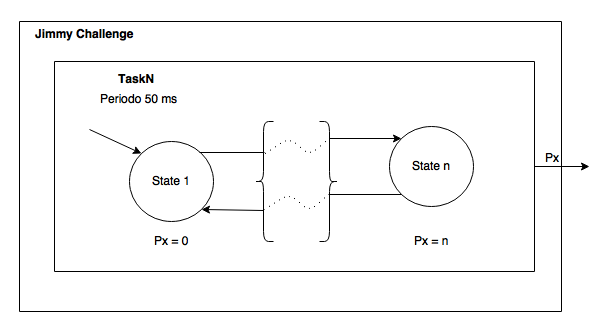
\includegraphics[scale=.40]{img/task_generic.png}
	\caption{Generalizzazione dei task}
\end{figure}

\clearpage
\section{Elenco dei Task sviluppati:}
\begin{enumerate}
	\item SonarTask
	\item ButtonTask
	\item BuzzerTask
	\item LedTask
	\item LedPwmTask
	\item LedRgbTask
\end{enumerate}

\subsection{SonarTask}
È il task più importante del progetto in quanto:
\begin{itemize}
	\item permette l'interazione utente-sistema sfruttando il sensore ad ultrasuoni;
	\item aggiorna la \texttt{currentDistance} del Context (\ref{sec:context});
	\item in modo indiretto può variare l'evoluzione del sistema
\end{itemize}
Nella classe SonarTask viene definito il metodo \texttt{playLevel()} in cui:
\begin{itemize}
	\item si legge la currentDistance dal sonar;
	\item si setta tale currentDistance nel Context;
	\item si gestiscono gli \texttt{status} da inviare alla seriale
\end{itemize}

Dal Context:
\begin{itemize}
	\item si riceve il \textbf{numero segreto}: la distanza del pistoncino a partire dal punto 0, ovvero il sonar);
	\item si riceve il \textbf{delta}: intervallo di errore in cui la posizione del pistoncino è considerata corretta;
	\item si riceve il \textbf{livello attuale} a cui si sta giocando;
	\item si controlla se il lucchetto è aperto con \texttt{pContext->isPadLockOpen()}
\end{itemize}
Sul Context:
\begin{itemize}
	\item se il lucchetto è stato aperto si crea un nuovo livello con \texttt{pContext->setNewLevel()};
	\item se il padLock non è stato completamente sbloccato viene settato come chiuso con \texttt{pContext->setPadlockOpen(false)};
	\item se il padLock non è stato completamente sbloccato viene resettato lo stato di scasso con \texttt{pContext->setLockpicking(false)};
	\item in base al tempo passato nello scassinare il lucchetto (e quindi allo \texttt{status} in cui ci si trova), viene settato \texttt{pContex->setDangerLevel(...)} con un numero da 0 a 4, (che nel LedRgbTask indica il colore da visualizzare sul LED RGB).
\end{itemize}
Per la rilevazione della distanza della mano dal sensore è stata utilizzata la libreria \textbf{NewPing} \ref{sec:newping}.
\begin{figure}[!ht]
	\centering
	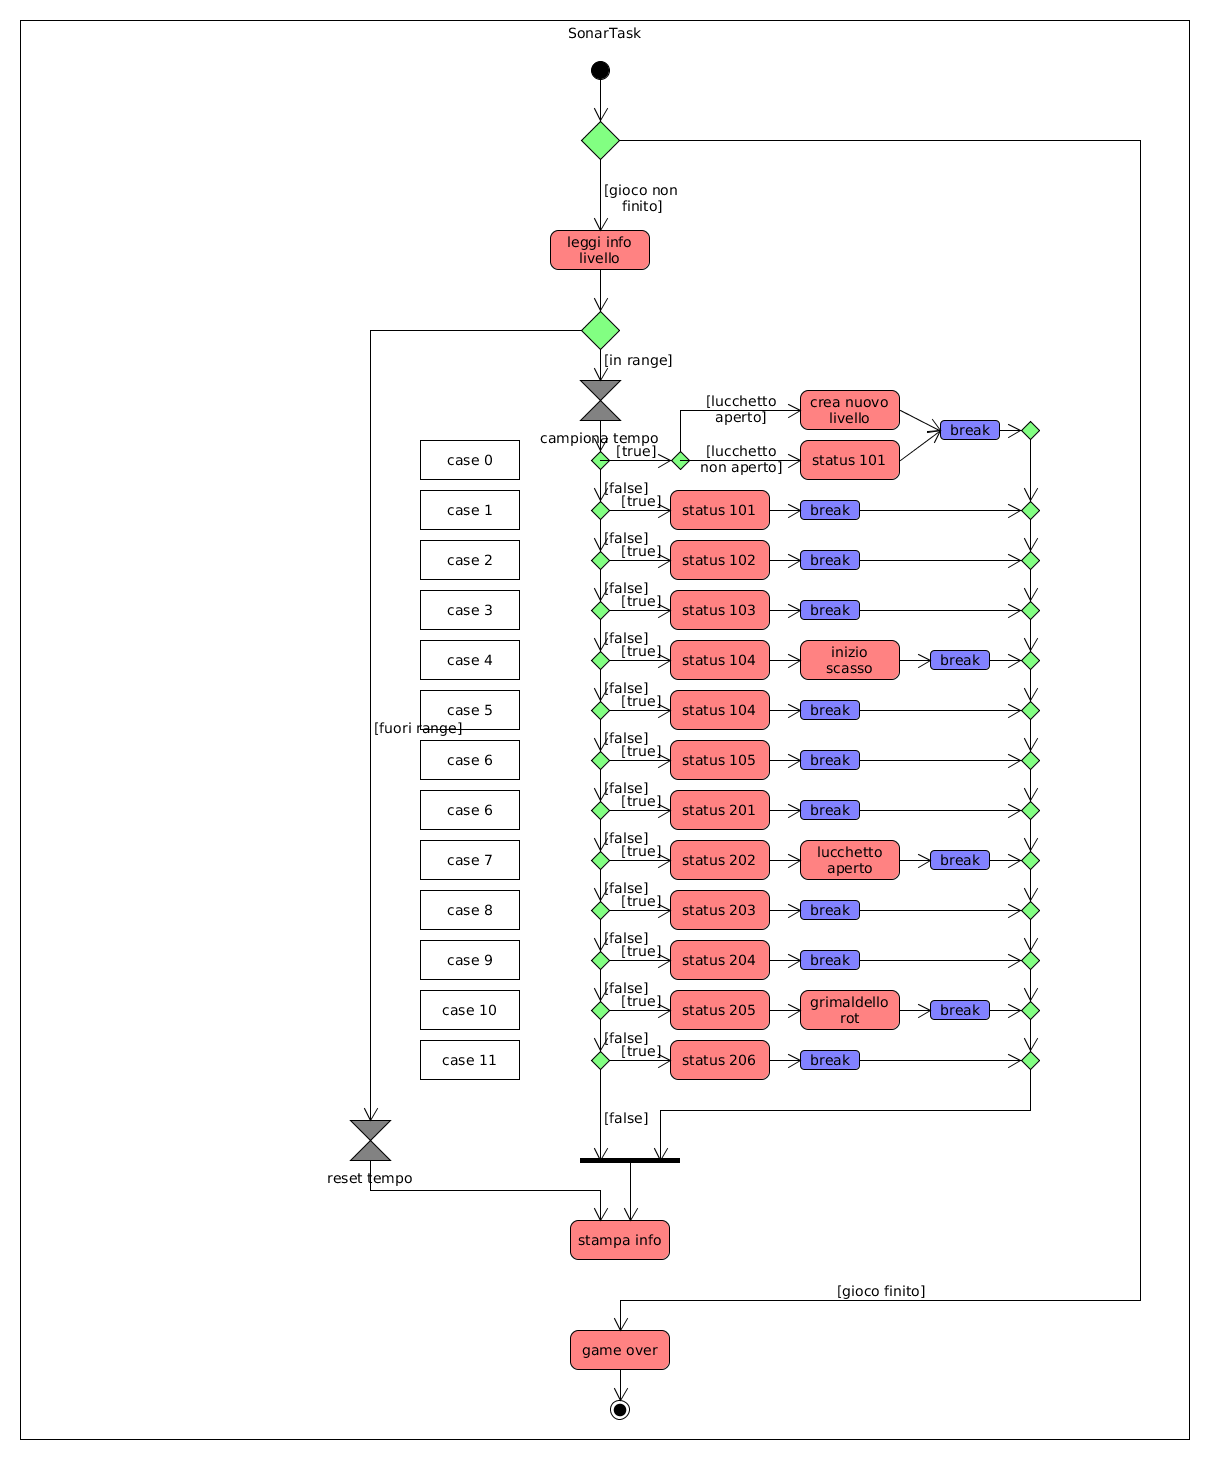
\includegraphics[scale=.35]{img/UML/sonartask.png}
	\caption{Diagramma di attività - playLevel()}
\end{figure}

\newpage
\subsection{ButtonTask}
Questo task controlla se è avvenuta la pressione del \textit{button}.
Finché il gioco non è finito è possibile stampare su terminale un messaggio che indica la posizione del lucchetto. 

Se il gioco è finito, ma il bottone viene comunque premuto, si avvia un divertente \textbf{\textit{easter egg}} legata al BuzzerTask e ad un famoso gioco degli anni '80\dots


\subsection{BuzzerTask}
Questo task controlla i suoni che il \textit{buzzer} deve emettere attraverso il metodo \texttt{playSound(<num>)}

\begin{itemize}
	\item Se il gioco non è finito e il lucchetto non è ancora stato trovato, viene emesso il suono 0;
	\item Se il gioco non è finito e il lucchetto è stato trovato, viene emesso il suono 1;
	\item Se il gioco è finito e il pulsante premuto, viene emesso il suono 2 (\textbf{\textit{easter egg}}).
\end{itemize}

\subsection{LedTask}
Questo task controlla l'accensione e lo spegnimento del LED verde.

\begin{itemize}
	\item Se il gioco non è finito e il lucchetto è stato trovato, il LED viene acceso;
	\item Se il gioco non è finito e il lucchetto non è ancora stato trovato, il LED viene spento.
\end{itemize}

\subsection{LedPwmTask}
Questo task gestisce il LED verde utilizzando il pin PWM grazie ai seguenti metodi:
\begin{itemize}
	\item \texttt{setIntensity(<num>)} per gestire l'intensità luminosa (anche temporizzata) del LED;
	\item \texttt{switchOff()} per spegnere immediatamente il LED.
\end{itemize}
Analizzando questo task nel dettaglio:
\begin{itemize}
	\item Se il lucchetto non è stato aperto e non è stato trovato:
	\begin{itemize}
		\item si aumenta l'intensità del LED usando un ciclo \texttt{for} inizializzato a 64 (in modo da non partire dal LED completamente spento) per arrivare a 255 (valore massimo consentito).
		\item al termine del ciclo il LED viene spento
	\end{itemize}
	L'obiettivo di questo frammento di codice è far capire al giocatore che il sistema è in funzione facendo illuminare e subito spegnere il LED, come se questo emettesse tanti flash luminosi.
	\item Se il gioco è finito:
	\begin{itemize}
		\item si aumenta l'intensità del LED usando un ciclo \texttt{for} inizializzato a 10 (riducendo il tempo necessario per arrivare al massimo).
		\item all'interno di questo ciclo è stato inserito un \textbf{delay} di 3 ms per rendere più visibile il dimmeraggio
		\item al termine del ciclo for, il LED viene spento.
	\end{itemize}
\end{itemize}

\subsection{LedRgbTask}
Questo task gestisce il funzionamento del LED RGB.

In fase di creazione prende in input i pin PWM dell'Arduino a cui è collegato fisicamente il LED RGB (costanti \texttt{LED\_RGB\_R}, \texttt{LED\_RGB\_G}, \texttt{LED\_RGB\_B}).

Funzionamento:
\begin{itemize}
	\item Finché il gioco non è finito:
	\begin{itemize}
		\item Se si è in fase di scasso, si imposta un colore nel costrutto swhitch-case in base al livello di pericolo di \texttt{getDangerLevel()}
			\item Nel dettaglio:
			\begin{itemize}
				\item 0 = \textbf{blu scuro} (inizio stato di scasso); 
				\item 1 = \textbf{verde} (lucchetto sbloccato);
				\item 2 = \textbf{giallo} (attenzione, rischio di rompere il grimaldello);
				\item 3 = \textbf{rosa} (attenzione, elevato pericolo di rottura);
				\item 4 = \textbf{rosso} (rottura del lucchetto).
			\end{itemize}
		\item Altrimenti si imposta un colore \textbf{\textit{light blue}} costante.
	\end{itemize}
\end{itemize}





